\documentclass[10.5pt,a4paper]{article}
\usepackage[a4paper,margin=2.1cm,top=2.0cm,bottom=2.2cm]{geometry}
\usepackage{fontspec}
\setmainfont{IBMPlexSans}[
  Path = ../fonts/,
  Extension = .ttf,
  UprightFont = *-Regular,
  ItalicFont = *-Italic,
  BoldFont = *-SemiBold,
  BoldItalicFont = *-Italic]
\setmonofont{IBMPlexMono}[
  Extension = .otf,
  UprightFont = *-Regular,
  ItalicFont = *-Italic,
  BoldFont = *-SemiBold,
  Scale = MatchLowercase]
\usepackage{unicode-math}
\setmathfont{IBMPlexMath-Regular.otf}
\usepackage{graphicx}
\graphicspath{{../figures/}{../slides/assets/}}
\usepackage{booktabs}
\usepackage{tabularx}
\usepackage{array}
\usepackage{multirow}
\usepackage[font=small,skip=5pt,justification=justified,singlelinecheck=false]{caption}
\usepackage{xcolor}
\definecolor{bnmuted}{HTML}{6B7280}
\definecolor{nusblue}{HTML}{003D7C}
\definecolor{nusorange}{HTML}{EF7C00}
\usepackage[colorlinks=true,linkcolor=black,urlcolor=black,citecolor=black]{hyperref}
\usepackage{enumitem}
\setlist{nosep,leftmargin=1.2em}
\usepackage{float}
\usepackage{flafter}
\setcounter{topnumber}{3}
\setcounter{totalnumber}{4}
\renewcommand{\topfraction}{0.9}
\renewcommand{\textfraction}{0.08}
\renewcommand{\floatpagefraction}{0.75}
\setlength{\textfloatsep}{12pt plus 3pt minus 2pt}
\setlength{\floatsep}{10pt plus 2pt minus 2pt}
\setlength{\intextsep}{10pt plus 2pt minus 2pt}
\makeatletter
\setlength{\@fptop}{0pt}
\setlength{\@fpsep}{14pt plus 2pt}
\setlength{\@fpbot}{0pt plus 1fil}
\makeatother
\usepackage{titlesec}
\setcounter{secnumdepth}{2}
\titleformat{\section}{\large\bfseries\color{nusblue}}{\thesection}{0.6em}{}
\titleformat{\subsection}{\normalsize\bfseries\color{nusblue}}{\thesubsection}{0.6em}{}
\titlespacing*{\section}{0pt}{14pt}{6pt}
\titlespacing*{\subsection}{0pt}{10pt}{4pt}
\usepackage{indentfirst}
\setlength{\parindent}{1.5em}
\setlength{\parskip}{0pt plus 1pt}
\linespread{1.08}
\usepackage{fancyhdr}
\pagestyle{fancy}
\fancyhf{}
\renewcommand{\headrulewidth}{0pt}
\fancyfoot[L]{\footnotesize\color{bnmuted}BN5211 Final Project, Topic 1: Surgical skill assessment from kinematics and video}
\fancyfoot[R]{\footnotesize\color{bnmuted}\thepage}
\usepackage[numbers,sort&compress]{natbib}
\setlength{\bibsep}{0pt}
\renewcommand{\bibfont}{\small}
\renewcommand{\bibsection}{\section{References}}

%% Team information (shared by the English and Chinese reports and slides).
%% Member names and student IDs are kept out of the public repository.
\newcommand{\GroupName}{Group 17}
\newcommand{\TeamMembers}{National University of Singapore}
\newcommand{\ReportDate}{November 2026}

%% generated by code/make_tables.py from results/results.json -- do not edit
\newcommand{\FMZero}{0.218}
\newcommand{\AccMZero}{0.487}
\newcommand{\AccPctMZero}{48.7}
\newcommand{\LoMZero}{0.074}
\newcommand{\HiMZero}{0.310}
\newcommand{\PMZero}{1.000}
\newcommand{\FNMZero}{0.66}
\newcommand{\FIMZero}{0.00}
\newcommand{\FEMZero}{0.00}
\newcommand{\FoldAccMZero}{0.50}
\newcommand{\FoldSdMZero}{0.53}
\newcommand{\UBMZero}{5/5}
\newcommand{\UCMZero}{0/5}
\newcommand{\UDMZero}{0/5}
\newcommand{\UEMZero}{0/5}
\newcommand{\UFMZero}{0/5}
\newcommand{\UGMZero}{5/5}
\newcommand{\UHMZero}{4/4}
\newcommand{\UIMZero}{5/5}
\newcommand{\FMOne}{0.515}
\newcommand{\AccMOne}{0.615}
\newcommand{\AccPctMOne}{61.5}
\newcommand{\LoMOne}{0.272}
\newcommand{\HiMOne}{0.618}
\newcommand{\PMOne}{0.033}
\newcommand{\FNMOne}{0.75}
\newcommand{\FIMOne}{0.64}
\newcommand{\FEMOne}{0.15}
\newcommand{\FoldAccMOne}{0.62}
\newcommand{\FoldSdMOne}{0.34}
\newcommand{\UBMOne}{4/5}
\newcommand{\UCMOne}{4/5}
\newcommand{\UDMOne}{1/5}
\newcommand{\UEMOne}{0/5}
\newcommand{\UFMOne}{4/5}
\newcommand{\UGMOne}{5/5}
\newcommand{\UHMOne}{3/4}
\newcommand{\UIMOne}{3/5}
\newcommand{\FMTwoA}{0.345}
\newcommand{\AccMTwoA}{0.436}
\newcommand{\AccPctMTwoA}{43.6}
\newcommand{\LoMTwoA}{0.125}
\newcommand{\HiMTwoA}{0.496}
\newcommand{\PMTwoA}{0.455}
\newcommand{\FNMTwoA}{0.72}
\newcommand{\FIMTwoA}{0.00}
\newcommand{\FEMTwoA}{0.32}
\newcommand{\FoldAccMTwoA}{0.45}
\newcommand{\FoldSdMTwoA}{0.50}
\newcommand{\UBMTwoA}{0/5}
\newcommand{\UCMTwoA}{0/5}
\newcommand{\UDMTwoA}{0/5}
\newcommand{\UEMTwoA}{3/5}
\newcommand{\UFMTwoA}{0/5}
\newcommand{\UGMTwoA}{5/5}
\newcommand{\UHMTwoA}{4/4}
\newcommand{\UIMTwoA}{5/5}
\newcommand{\FMTwoB}{0.371}
\newcommand{\AccMTwoB}{0.487}
\newcommand{\AccPctMTwoB}{48.7}
\newcommand{\LoMTwoB}{0.222}
\newcommand{\HiMTwoB}{0.467}
\newcommand{\PMTwoB}{0.348}
\newcommand{\FNMTwoB}{0.75}
\newcommand{\FIMTwoB}{0.36}
\newcommand{\FEMTwoB}{0.00}
\newcommand{\FoldAccMTwoB}{0.49}
\newcommand{\FoldSdMTwoB}{0.38}
\newcommand{\UBMTwoB}{4/5}
\newcommand{\UCMTwoB}{3/5}
\newcommand{\UDMTwoB}{0/5}
\newcommand{\UEMTwoB}{0/5}
\newcommand{\UFMTwoB}{1/5}
\newcommand{\UGMTwoB}{5/5}
\newcommand{\UHMTwoB}{3/4}
\newcommand{\UIMTwoB}{3/5}
\newcommand{\FMTwoC}{0.420}
\newcommand{\AccMTwoC}{0.513}
\newcommand{\AccPctMTwoC}{51.3}
\newcommand{\LoMTwoC}{0.178}
\newcommand{\HiMTwoC}{0.576}
\newcommand{\PMTwoC}{0.240}
\newcommand{\FNMTwoC}{0.67}
\newcommand{\FIMTwoC}{0.59}
\newcommand{\FEMTwoC}{0.00}
\newcommand{\FoldAccMTwoC}{0.50}
\newcommand{\FoldSdMTwoC}{0.47}
\newcommand{\UBMTwoC}{5/5}
\newcommand{\UCMTwoC}{5/5}
\newcommand{\UDMTwoC}{0/5}
\newcommand{\UEMTwoC}{0/5}
\newcommand{\UFMTwoC}{3/5}
\newcommand{\UGMTwoC}{5/5}
\newcommand{\UHMTwoC}{0/4}
\newcommand{\UIMTwoC}{2/5}
\newcommand{\FMThree}{0.443}
\newcommand{\AccMThree}{0.538}
\newcommand{\AccPctMThree}{53.8}
\newcommand{\LoMThree}{0.247}
\newcommand{\HiMThree}{0.568}
\newcommand{\PMThree}{0.188}
\newcommand{\FNMThree}{0.75}
\newcommand{\FIMThree}{0.45}
\newcommand{\FEMThree}{0.12}
\newcommand{\FoldAccMThree}{0.54}
\newcommand{\FoldSdMThree}{0.36}
\newcommand{\UBMThree}{4/5}
\newcommand{\UCMThree}{4/5}
\newcommand{\UDMThree}{1/5}
\newcommand{\UEMThree}{0/5}
\newcommand{\UFMThree}{1/5}
\newcommand{\UGMThree}{5/5}
\newcommand{\UHMThree}{3/4}
\newcommand{\UIMThree}{3/5}
\newcommand{\FMThreeB}{0.450}
\newcommand{\AccMThreeB}{0.538}
\newcommand{\AccPctMThreeB}{53.8}
\newcommand{\LoMThreeB}{0.253}
\newcommand{\HiMThreeB}{0.567}
\newcommand{\PMThreeB}{0.133}
\newcommand{\FNMThreeB}{0.72}
\newcommand{\FIMThreeB}{0.50}
\newcommand{\FEMThreeB}{0.13}
\newcommand{\FoldAccMThreeB}{0.54}
\newcommand{\FoldSdMThreeB}{0.33}
\newcommand{\UBMThreeB}{3/5}
\newcommand{\UCMThreeB}{2/5}
\newcommand{\UDMThreeB}{1/5}
\newcommand{\UEMThreeB}{0/5}
\newcommand{\UFMThreeB}{4/5}
\newcommand{\UGMThreeB}{5/5}
\newcommand{\UHMThreeB}{3/4}
\newcommand{\UIMThreeB}{3/5}
\newcommand{\FMThreeC}{0.481}
\newcommand{\AccMThreeC}{0.615}
\newcommand{\AccPctMThreeC}{61.5}
\newcommand{\LoMThreeC}{0.236}
\newcommand{\HiMThreeC}{0.596}
\newcommand{\PMThreeC}{0.062}
\newcommand{\FNMThreeC}{0.75}
\newcommand{\FIMThreeC}{0.69}
\newcommand{\FEMThreeC}{0.00}
\newcommand{\FoldAccMThreeC}{0.62}
\newcommand{\FoldSdMThreeC}{0.40}
\newcommand{\UBMThreeC}{4/5}
\newcommand{\UCMThreeC}{4/5}
\newcommand{\UDMThreeC}{0/5}
\newcommand{\UEMThreeC}{0/5}
\newcommand{\UFMThreeC}{5/5}
\newcommand{\UGMThreeC}{5/5}
\newcommand{\UHMThreeC}{3/4}
\newcommand{\UIMThreeC}{3/5}
\newcommand{\FMThreeD}{0.461}
\newcommand{\AccMThreeD}{0.615}
\newcommand{\AccPctMThreeD}{61.5}
\newcommand{\LoMThreeD}{0.242}
\newcommand{\HiMThreeD}{0.564}
\newcommand{\PMThreeD}{0.036}
\newcommand{\FNMThreeD}{0.74}
\newcommand{\FIMThreeD}{0.64}
\newcommand{\FEMThreeD}{0.00}
\newcommand{\FoldAccMThreeD}{0.62}
\newcommand{\FoldSdMThreeD}{0.41}
\newcommand{\UBMThreeD}{4/5}
\newcommand{\UCMThreeD}{4/5}
\newcommand{\UDMThreeD}{0/5}
\newcommand{\UEMThreeD}{0/5}
\newcommand{\UFMThreeD}{4/5}
\newcommand{\UGMThreeD}{5/5}
\newcommand{\UHMThreeD}{4/4}
\newcommand{\UIMThreeD}{3/5}
\newcommand{\FMFour}{0.520}
\newcommand{\AccMFour}{0.615}
\newcommand{\AccPctMFour}{61.5}
\newcommand{\LoMFour}{0.273}
\newcommand{\HiMFour}{0.619}
\newcommand{\PMFour}{0.074}
\newcommand{\FNMFour}{0.75}
\newcommand{\FIMFour}{0.67}
\newcommand{\FEMFour}{0.14}
\newcommand{\FoldAccMFour}{0.61}
\newcommand{\FoldSdMFour}{0.35}
\newcommand{\UBMFour}{4/5}
\newcommand{\UCMFour}{4/5}
\newcommand{\UDMFour}{1/5}
\newcommand{\UEMFour}{0/5}
\newcommand{\UFMFour}{4/5}
\newcommand{\UGMFour}{5/5}
\newcommand{\UHMFour}{2/4}
\newcommand{\UIMFour}{4/5}
\newcommand{\FMFive}{0.440}
\newcommand{\AccMFive}{0.538}
\newcommand{\AccPctMFive}{53.8}
\newcommand{\LoMFive}{0.259}
\newcommand{\HiMFive}{0.526}
\newcommand{\PMFive}{0.157}
\newcommand{\FNMFive}{0.73}
\newcommand{\FIMFive}{0.45}
\newcommand{\FEMFive}{0.13}
\newcommand{\FoldAccMFive}{0.54}
\newcommand{\FoldSdMFive}{0.33}
\newcommand{\UBMFive}{4/5}
\newcommand{\UCMFive}{3/5}
\newcommand{\UDMFive}{1/5}
\newcommand{\UEMFive}{0/5}
\newcommand{\UFMFive}{2/5}
\newcommand{\UGMFive}{5/5}
\newcommand{\UHMFive}{3/4}
\newcommand{\UIMFive}{3/5}
\newcommand{\FCOne}{0.375}
\newcommand{\AccCOne}{0.487}
\newcommand{\AccPctCOne}{48.7}
\newcommand{\LoCOne}{0.275}
\newcommand{\HiCOne}{0.482}
\newcommand{\PCOne}{0.367}
\newcommand{\FNCOne}{0.82}
\newcommand{\FICOne}{0.20}
\newcommand{\FECOne}{0.11}
\newcommand{\FoldAccCOne}{0.50}
\newcommand{\FoldSdCOne}{0.41}
\newcommand{\UBCOne}{4/5}
\newcommand{\UCCOne}{2/5}
\newcommand{\UDCOne}{0/5}
\newcommand{\UECOne}{1/5}
\newcommand{\UFCOne}{0/5}
\newcommand{\UGCOne}{3/5}
\newcommand{\UHCOne}{4/4}
\newcommand{\UICOne}{5/5}
\newcommand{\FCTwo}{0.342}
\newcommand{\AccCTwo}{0.385}
\newcommand{\AccPctCTwo}{38.5}
\newcommand{\LoCTwo}{0.167}
\newcommand{\HiCTwo}{0.475}
\newcommand{\PCTwo}{0.445}
\newcommand{\FNCTwo}{0.47}
\newcommand{\FICTwo}{0.43}
\newcommand{\FECTwo}{0.12}
\newcommand{\FoldAccCTwo}{0.38}
\newcommand{\FoldSdCTwo}{0.31}
\newcommand{\UBCTwo}{3/5}
\newcommand{\UCCTwo}{4/5}
\newcommand{\UDCTwo}{1/5}
\newcommand{\UECTwo}{0/5}
\newcommand{\UFCTwo}{1/5}
\newcommand{\UGCTwo}{4/5}
\newcommand{\UHCTwo}{1/4}
\newcommand{\UICTwo}{1/5}
\newcommand{\FCTwoT}{0.344}
\newcommand{\AccCTwoT}{0.385}
\newcommand{\AccPctCTwoT}{38.5}
\newcommand{\LoCTwoT}{0.132}
\newcommand{\HiCTwoT}{0.509}
\newcommand{\PCTwoT}{0.371}
\newcommand{\FNCTwoT}{0.38}
\newcommand{\FICTwoT}{0.53}
\newcommand{\FECTwoT}{0.12}
\newcommand{\FoldAccCTwoT}{0.38}
\newcommand{\FoldSdCTwoT}{0.37}
\newcommand{\UBCTwoT}{1/5}
\newcommand{\UCCTwoT}{5/5}
\newcommand{\UDCTwoT}{1/5}
\newcommand{\UECTwoT}{0/5}
\newcommand{\UFCTwoT}{3/5}
\newcommand{\UGCTwoT}{4/5}
\newcommand{\UHCTwoT}{1/4}
\newcommand{\UICTwoT}{0/5}
\newcommand{\DOneZero}{$+$0.296}
\newcommand{\DAbsOneZero}{0.296}
\newcommand{\DLoOneZero}{$+$0.015}
\newcommand{\DHiOneZero}{$+$0.443}
\newcommand{\DThreeOne}{$-$0.071}
\newcommand{\DAbsThreeOne}{0.071}
\newcommand{\DLoThreeOne}{$-$0.170}
\newcommand{\DHiThreeOne}{$+$0.010}
\newcommand{\DFourOne}{$+$0.005}
\newcommand{\DAbsFourOne}{0.005}
\newcommand{\DLoFourOne}{$-$0.043}
\newcommand{\DHiFourOne}{$+$0.051}
\newcommand{\DThreeBOne}{$-$0.064}
\newcommand{\DAbsThreeBOne}{0.064}
\newcommand{\DLoThreeBOne}{$-$0.133}
\newcommand{\DHiThreeBOne}{$+$0.000}
\newcommand{\DThreeCOne}{$-$0.034}
\newcommand{\DAbsThreeCOne}{0.034}
\newcommand{\DLoThreeCOne}{$-$0.111}
\newcommand{\DHiThreeCOne}{$+$0.050}
\newcommand{\DThreeDOne}{$-$0.053}
\newcommand{\DAbsThreeDOne}{0.053}
\newcommand{\DLoThreeDOne}{$-$0.128}
\newcommand{\DHiThreeDOne}{$+$0.019}
\newcommand{\DFiveFour}{$-$0.080}
\newcommand{\DAbsFiveFour}{0.080}
\newcommand{\DLoFiveFour}{$-$0.128}
\newcommand{\DHiFiveFour}{$+$0.014}
\newcommand{\DTwoBZero}{$+$0.153}
\newcommand{\DAbsTwoBZero}{0.153}
\newcommand{\DLoTwoBZero}{$-$0.020}
\newcommand{\DHiTwoBZero}{$+$0.259}
\newcommand{\IdKSimple}{0.92}
\newcommand{\IdKTexture}{0.89}
\newcommand{\IdDuration}{0.26}
\newcommand{\IdVAppear}{1.00}
\newcommand{\IdVDyn}{0.44}
\newcommand{\IdVFlow}{0.56}
\newcommand{\NTrials}{39}
\newcommand{\DurMin}{59}
\newcommand{\DurMax}{300}
\newcommand{\DurMedian}{105}
\newcommand{\DurN}{124}
\newcommand{\DurI}{84}
\newcommand{\DurE}{89}
\newcommand{\NFramesOneHz}{4406}
\newcommand{\NPairsTwoHz}{8794}
\newcommand{\PaceKSimple}{0.42}
\newcommand{\PaceVDyn}{0.54}
\newcommand{\PaceKTexture}{0.34}
\newcommand{\PaceVFlow}{0.35}
\newcommand{\PaceKTextureMax}{0.93}
\newcommand{\VerPython}{3.11.0}
\newcommand{\VerNumpy}{2.4.6}
\newcommand{\VerSklearn}{1.9.1}
\newcommand{\VerTorch}{2.11.0+cu128}
\newcommand{\VerTorchvision}{0.26.0+cu128}
\newcommand{\VerOpencv}{5.0.0}
\newcommand{\VerScipy}{1.17.1}
\newcommand{\VerPandas}{3.0.5}
\newcommand{\CaseGZeroOneDur}{300}
\newcommand{\CaseGZeroOnePPred}{0.98}
\newcommand{\CaseGZeroOnePTrue}{0.98}
\newcommand{\CaseCZeroFourDur}{83}
\newcommand{\CaseCZeroFourPPred}{0.91}
\newcommand{\CaseCZeroFourPTrue}{0.91}
\newcommand{\CaseEZeroOneDur}{120}
\newcommand{\CaseEZeroOnePPred}{0.69}
\newcommand{\CaseEZeroOnePTrue}{0.14}
\newcommand{\CaseDZeroFiveDur}{59}
\newcommand{\CaseDZeroFivePPred}{0.89}
\newcommand{\CaseDZeroFivePTrue}{0.04}
\newcommand{\CaseIZeroFiveDur}{126}
\newcommand{\CaseIZeroFivePPred}{0.93}
\newcommand{\CaseIZeroFivePTrue}{0.07}
\newcommand{\DurRangeD}{59--93}
\newcommand{\DurRangeE}{83--120}
\newcommand{\DurRangeCF}{68--109}

\newcommand{\pp}{\,pp}

\begin{document}
\noindent
\includegraphics[height=1.25cm]{NationalUniversityofSingapore.pdf}\par
\vspace{2pt}{\color{nusorange}\rule{\textwidth}{1.2pt}}\par\vspace{6pt}
\begin{center}
{\LARGE\bfseries\color{nusblue} Surgical Skill Assessment from Kinematics and Video}\\[3pt]
{\large Classifying novice, intermediate and expert surgeons on JIGSAWS Suturing under leave-one-user-out evaluation}\\[8pt]
{\normalsize BN5211 Medical Robotic Intelligence, Final Project (Topic 1)\quad\textbar\quad \GroupName}\\[4pt]
{\small \TeamMembers}\\[2pt]
{\small\color{bnmuted} \ReportDate}
\end{center}
\vspace{2pt}
% the title and team block is item 1 of the required report structure, so Background is Section 2
\setcounter{section}{1}

\section{Background}

\subsection{Clinical and robotic motivation}

Technical skill matters clinically. In a study of bariatric surgeons whose operating videos were rated by peers, the lowest-rated quartile had markedly higher rates of complications, reoperation and readmission than the highest-rated quartile \citep{birkmeyer2013skill}. Skill is still assessed mainly by expert observers with structured checklists and global rating scales such as OSATS \citep{martin1997osats}. That process is slow, expensive and partly subjective, so it is hard to give trainees frequent feedback or to apply it consistently for credentialing \citep{reiley2011review}. Robot-assisted minimally invasive surgery changes the situation because the robot already records what the surgeon does. The da~Vinci system logs the pose, velocity and gripper angle of every manipulator at a fixed rate, and the endoscope records the operative field. Objective skill assessment can therefore be computed from data that are collected anyway, which makes it a natural problem for medical robotic intelligence. A model of this kind is only useful in practice if it works for a surgeon it has never seen. A trainee who is assessed by such a system will not have contributed trials to its training set, so the evaluation has to hold out whole surgeons rather than individual trials.

\subsection{Related work}

The JHU-ISI Gesture and Skill Assessment Working Set (JIGSAWS) is the standard public benchmark for this problem \citep{gao2014jigsaws}. It contains synchronised kinematics and stereo video of eight surgeons who each performed suturing, knot tying and needle passing on a bench-top model, together with a self-reported skill level and a modified OSATS score per trial. Benchmark protocols for the dataset distinguish leave-one-supertrial-out (LOSO), in which one repetition of every surgeon is held out, from leave-one-user-out (LOUO), in which all trials of one surgeon are held out \citep{ahmidi2017benchmarks}. Kinematic approaches fall roughly into three groups. The first summarises a trial with global motion statistics such as completion time, path length, economy of motion and the number of gripper movements, which are close to the metrics that expert raters use and are cheap to compute \citep{reiley2011review, lefor2020motion, anh2020features}. The second describes the texture of the motion signal. \citet{zia2018rmis}, the background reference of this topic, computed approximate entropy \citep{pincus1991apen} and related measures on every kinematic channel and reported 88.2\% accuracy for Suturing under LOUO with a nearest-neighbour classifier, and the same group applied the idea to video and accelerometer data \citep{zia2018video}. The third learns features end-to-end, for example with convolutional networks on the raw kinematic sequence \citep{fawaz2018cnn, wang2018cnn} or on video clips \citep{funke2019video, liu2021unified}, and recent video transformers decode surgeon activity and skill from clinical recordings \citep{kiyasseh2023vit, lavanchy2021threestage}. Many of the highest published numbers use LOSO, in which every test surgeon also appears in the training set, and accuracies near 100\% are common under that split \citep{fawaz2018cnn, funke2019video}. Under LOUO the task becomes generalisation to new people from only seven training surgeons, and the uncertainty of any estimate is large \citep{varoquaux2018cv}. Results obtained under the two splits are therefore not comparable. The class distribution adds a second difficulty. Novices contribute almost half of the Suturing trials, so accuracy rewards a classifier that favours the majority class, and the literature on imbalanced learning recommends class-balanced training together with metrics that weight every class equally, such as macro-F1 \citep{he2009imbalanced}. We follow both recommendations.

\subsection{Motivation for the approach}

The topic prescribes the core experiment: a kinematics-only baseline built from simple trial-level statistics, video features from sampled frames or short clips, a simple fusion of the two, and a comparison with the majority class under LOUO with macro-F1. Our design choices follow from two properties of the data. First, JIGSAWS Suturing has 39 usable trials from eight surgeons, and the skill label is constant within a surgeon. The effective sample size for learning what distinguishes skill levels is therefore closer to eight than to 39, with only two surgeons in each of the intermediate and expert classes. This favours low-capacity models with few free parameters and strong regularisation over end-to-end deep networks, and we use frozen pretrained image features with a linear classifier rather than any fine-tuning. Second, because labels belong to surgeons, any feature that identifies the surgeon also predicts the label inside the training set without capturing skill. We therefore treat shortcut detection as part of the method and add two measurements to the required experiment: a probe of how strongly each feature block encodes surgeon identity, and controls that measure how much of the decision is explained by the pace of the trial. As the focused improvement we test the central idea of the background reference, namely that expertise shows in the regularity of movement rather than only in its speed, by adding motion-texture features to the simple statistics. All models, metrics and comparisons were fixed in a written protocol before the first result was computed, so that the choice of the reported model could not be influenced by the outcome.

\section{Methods}

\subsection{Data and task}

We use the Suturing task of the official JIGSAWS release. The metadata file lists \NTrials{} trials from eight surgeons (users B to I). Each user performed five trials, except user H, whose trial H002 has no label or fold entry in the official release and is therefore absent. The target is the self-reported skill level, novice (N, under 10 hours of robotic practice), intermediate (I, 10 to 100 hours) or expert (E, over 100 hours). Users B, G, H and I are novices (19 trials), C and F intermediates (10 trials), and D and E experts (10 trials). Each trial provides 76 kinematic channels sampled at 30\,Hz, namely the Cartesian position, rotation matrix, linear velocity, angular velocity and gripper angle of the two surgeon-side master manipulators and the two patient-side instruments, and two endoscope videos at 640$\times$480 pixels and 30 frames per second. We use the patient-side instruments for the kinematic features, because they are the tools that act on the tissue and the master signals largely duplicate them under teleoperation, and we use the left camera view (capture1) for the video features. Trials last between \DurMin{} and \DurMax{}\,s (median \DurMedian{}\,s), and novices are slower on average (Figure~\ref{fig:data}). Neither the gesture transcriptions nor the OSATS scores are used by any model.

\begin{figure}[htbp]
\centering
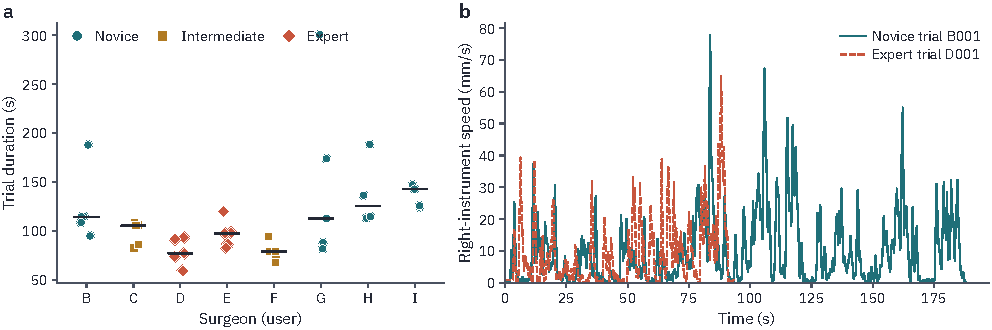
\includegraphics{fig2_data.pdf}
\caption{(a) Trial duration per surgeon, coloured by skill level; bars mark the median. (b) Speed of the right patient-side instrument, smoothed over 0.5\,s, in a novice trial (B001) and an expert trial (D001). The expert finishes in about half the time with a comparable peak speed.}
\label{fig:data}
\end{figure}

\subsection{Workflow}

Figure~\ref{fig:pipeline} summarises the pipeline. Each trial is turned into fixed-length feature vectors, one per feature block. A block is classified by a standardised, L2-regularised logistic regression whose regularisation strength is chosen inside the training surgeons. Multimodal models either concatenate blocks before classification (early fusion) or average the class probabilities of a kinematic and a video classifier (late fusion). Everything is evaluated with the eight official LOUO folds of the JIGSAWS skill-detection setup.

\begin{figure}[htbp]
\centering
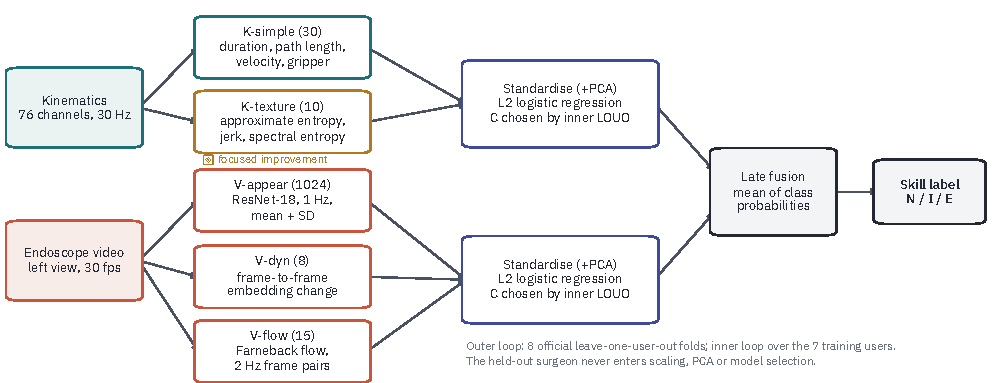
\includegraphics{fig1_pipeline.pdf}
\caption{Workflow. Kinematic and video feature blocks are extracted per trial and classified by regularised logistic regression; late fusion averages the class probabilities of one kinematic and one video classifier. The K-texture block is the focused improvement. Numbers in brackets are feature dimensions. All fitting, including scaling, PCA and the choice of the regularisation strength, uses only the training surgeons of each fold.}
\label{fig:pipeline}
\end{figure}

\subsection{Kinematic features}

The kinematics-only baseline (K-simple, 30 features) implements the statistics named in the task specification. For each patient-side instrument we compute the path length as the summed distance between consecutive tool-tip positions; the mean, standard deviation and 90th percentile of the linear speed; the mean and standard deviation of the angular speed; the idle fraction, defined as the share of samples with linear speed below 5\,mm/s; the economy of motion, defined as path length divided by the diagonal of the bounding box of the tool-tip trajectory; and five gripper statistics, namely the mean, standard deviation and range of the gripper angle, its total absolute change and the number of opening-and-closing cycles, counted as upward crossings of the mean of a 0.5\,s moving average. Four trial-level features complete the block: the duration in seconds, the correlation between the speeds of the two instruments, the share of time in which both are idle, and the log ratio of the two path lengths. All are standard descriptors of efficiency and bimanual coordination \citep{reiley2011review, lefor2020motion}.

The motion-texture block (K-texture, 10 features) is the focused improvement and follows the background reference \citep{zia2018rmis}. For each instrument we compute approximate entropy \citep{pincus1991apen} of the linear speed, the angular speed and the gripper angle, each resampled to 10\,Hz, with embedding dimension $m = 2$ and tolerance $r = 0.2$ times the standard deviation of the signal; the log dimensionless jerk of the velocity profile \citep{hogan2009smoothness}; and the normalised spectral entropy of the speed. These features describe how regular and smooth a movement is rather than how fast or how long, which is the property that should separate a fluent expert from a hesitant novice even when both take a similar time.

\subsection{Video features}

Frames are decoded once per trial. Every 30th frame (1\,Hz, \NFramesOneHz{} frames in total) is resized to 224$\times$224 pixels and passed through an ImageNet-pretrained ResNet-18 \citep{he2016resnet} with the classification layer removed, giving a 512-dimensional embedding per frame. The appearance block (V-appear, 1024 features) is the mean and the standard deviation of these embeddings over the trial; because 1024 dimensions are far too many for 34 training trials, a PCA with 4, 8 or 16 components is fitted inside each training fold. The scene-dynamics block (V-dyn, 8 features) summarises how fast the view changes: from the cosine distance between consecutive 1\,Hz embeddings we take the mean, standard deviation, 10th, 50th and 90th percentiles and coefficient of variation, and from the Euclidean distance the mean and standard deviation. A constant appearance offset, such as the lighting or the layout of the practice board in a given session, cancels in these differences, so V-dyn should carry less information about the recording setup than V-appear while still reflecting instrument motion and tissue change. The optical-flow block (V-flow, 15 features) uses Farneback dense flow \citep{farneback2003flow} on pairs of consecutive frames sampled at 2\,Hz (\NPairsTwoHz{} pairs) and downscaled to 320$\times$240 pixels. For each pair we compute the mean, standard deviation and 90th percentile of the flow magnitude, the fraction of pixels moving faster than 0.5 pixels per frame, and the magnitude-weighted entropy of the flow direction over eight bins, and we summarise each of these five series over the trial by its mean, standard deviation and 90th percentile.

\subsection{Classifiers and fusion}

Every block is classified by the same model: standardisation, optional PCA (V-appear only), a second standardisation after PCA, and multinomial logistic regression with an L2 penalty, balanced class weights and the L-BFGS solver \citep{pedregosa2011sklearn}. The inverse regularisation strength $C$ is chosen from $\{0.01, 0.03, 0.1, 0.3, 1, 3, 10\}$ and, for V-appear, the number of components from $\{4, 8, 16\}$. Late fusion averages the class probabilities of the kinematic classifier and one video classifier with equal weights; equal weighting was chosen because 34 training trials are too few to estimate a fusion weight reliably. Early fusion concatenates K-simple with V-dyn and fits one classifier. The primary multimodal model, fixed before any result was seen, is the late fusion of K-simple and V-dyn (M3). V-dyn was chosen as the primary video block for the first-principles reason given above and because an earlier exploratory analysis by our group on the same 39 trials had found embedding-change statistics to be the most promising video descriptor. Since that earlier analysis looked at out-of-fold results on the same data, the choice is not free of selection, and we therefore report all three video blocks and all four fusion variants.

\subsection{Evaluation protocol}

We use the official JIGSAWS folds in \texttt{Suturing/unBalanced/SkillDetection/UserOut}; the code checks that each fold holds out exactly one surgeon, which gives eight folds with 34 or 35 training trials. Hyperparameters are selected by an inner LOUO loop over the seven training surgeons of each outer fold, maximising the inner pooled macro-F1, with ties resolved towards stronger regularisation. When the outer fold holds out an intermediate or expert surgeon, only one surgeon of that class remains, and the inner fold that would hold it out has no training example of the class; such inner folds are skipped (one per affected outer fold). The held-out surgeon therefore never influences standardisation, PCA, feature residualisation or model selection.

The primary metric is macro-F1 computed once over the 39 pooled out-of-fold predictions. Because the label is constant within a surgeon, each LOUO test fold contains a single class and per-fold macro-F1 is undefined for the two absent classes, so pooling is the only well-defined form of the metric. We also report accuracy, per-class F1, the confusion matrix and accuracy per surgeon. With eight surgeons the uncertainty is large, so we quantify it in two ways that respect the grouping of trials. A user-level bootstrap resamples the eight surgeons with replacement 2000 times and gives percentile intervals for macro-F1 and for paired differences between models. An exact permutation test reassigns the skill labels among the surgeons while keeping each surgeon's trials together; with four novice, two intermediate and two expert surgeons there are $8!/(4!\,2!\,2!) = 420$ distinct assignments, so the null distribution of macro-F1 for fixed predictions is enumerated exactly and the smallest attainable $p$-value is $1/420$. Three comparisons were declared in advance: kinematics against the majority class (M1 vs M0), adding video to kinematics (M3 vs M1) and adding motion texture (M4 vs M1). A difference is called supported only if its bootstrap interval excludes zero. The complete protocol, including the model list in Table~\ref{tab:main}, was written to \texttt{PROTOCOL.md} before the pipeline was run, and every model was evaluated exactly once.

\subsection{Shortcut audit}

Two kinds of shortcut are plausible here. A feature block can identify the surgeon, in which case a classifier can reproduce training labels by recognising people, and that ability does not transfer to an unseen surgeon. We measure this with an identity probe: an eight-way surgeon classifier on each block, evaluated with stratified five-fold cross-validation over trials, whose balanced accuracy is compared with the chance level of 1/8. The second shortcut is pace. Novices are slower on average, so a model may rank trials by duration and call the result skill. We test this with a duration-only classifier (C1) and with K-simple after every feature has been residualised on log duration (C2, and C2t for the block with texture), with the regression fitted on the training surgeons only.

\subsection{Differences from existing work}
\label{sec:differences}

Our approach differs from the background reference and most related work in four ways. First, the reported numbers come from a protocol fixed before the run: every model, metric and comparison was written down in advance and each model was evaluated once, so the choice of the reported model could not depend on the test results. Second, we treat the eight surgeons rather than the 39 trials as the unit of uncertainty, reporting user-level bootstrap intervals and an exact permutation test over all 420 label assignments instead of a single accuracy, and we report macro-F1 so that the two small classes count as much as the novices. Third, we measure two shortcuts directly, the surgeon identity carried by each feature block and the share of the decision explained by trial duration, instead of assuming that a high score reflects skill. Fourth, the scene-dynamics descriptor V-dyn is designed to cancel the static appearance of a recording session, which whole-frame appearance features retain, and we test directly whether this reduces the identity shortcut.

\subsection{External resources and our contribution}

We used the JIGSAWS data and its official split files, the ImageNet weights of ResNet-18 distributed with torchvision \citep{paszke2019pytorch}, the Farneback implementation of OpenCV \citep{bradski2000opencv}, and scikit-learn \citep{pedregosa2011sklearn}, NumPy \citep{harris2020numpy} and SciPy \citep{virtanen2020scipy} for the classifiers and signal processing. No released skill-assessment code was used. The group implemented the data loading and fold checks, all feature definitions, the nested LOUO evaluation, the fusion models, the bootstrap and exact permutation analyses, the shortcut audit and all figures.

\section{Experiments and results}

\subsection{Experimental setup}

All experiments ran locally on one laptop with an NVIDIA GeForce RTX 3060 Laptop GPU (6\,GB) under Windows~11, with Python \VerPython{}, NumPy \VerNumpy{}, scikit-learn \VerSklearn{}, SciPy \VerScipy{}, PyTorch \VerTorch{}, torchvision \VerTorchvision{} and OpenCV \VerOpencv{}. Feature extraction for the 39 trials took about three minutes, dominated by optical flow, and the evaluation of all models including the bootstrap and permutation analyses took under two minutes. Every randomised step uses seed 0. Before the full run, the feature extractors were checked on a single trial (B001), which confirmed the frame counts, the alignment of the 5635 kinematic samples with the 5640 video frames, and the official fold membership. The full pipeline was then run once, and every number in this report is read from its output file.

\subsection{Quantitative results}

Table~\ref{tab:main} and Figure~\ref{fig:results} give the results of all models. The majority-class baseline always predicts novice, which is right for 19 of 39 trials (accuracy \AccMZero{}) and gives macro-F1 \FMZero{}, because the intermediate and expert classes receive F1 of zero. The kinematics-only baseline K-simple (M1) reaches macro-F1 \FMOne{} (95\% interval \LoMOne{} to \HiMOne{}) and accuracy \AccMOne{}. Its paired difference from the majority class is \DOneZero{} with interval \DLoOneZero{} to \DHiOneZero{}, which excludes zero, and the exact permutation test gives $p = \PMOne{}$. The first pre-declared comparison is therefore supported: simple trial statistics carry skill information that transfers to unseen surgeons, although the lower end of the interval is close to the majority level.

\begin{table}[htbp]
\centering
\small
\caption{Leave-one-user-out results on JIGSAWS Suturing (39 trials, 8 surgeons). Macro-F1, accuracy and per-class F1 are computed over the pooled out-of-fold predictions. The interval is the 2.5th to 97.5th percentile of 2000 user-level bootstrap resamples; $p$ is the exact user-level permutation $p$-value over all 420 label assignments. Bold rows are the kinematic baseline, the primary multimodal model and the focused improvement.}
\label{tab:main}
\begin{tabular}{@{}l l c c c c c c@{}}
\toprule
Model & ID & Macro-F1 [95\% CI] & Acc. & F1$_\mathrm{N}$ & F1$_\mathrm{I}$ & F1$_\mathrm{E}$ & $p$ \\
\midrule
\multicolumn{8}{@{}l}{\textit{Required experiment}} \\
\quad Majority class & M0 & 0.218 [0.074, 0.310] & 0.487 & 0.66 & 0.00 & 0.00 & 1.000 \\
\quad K-simple & M1 & \textbf{0.515} [0.272, 0.618] & 0.615 & 0.75 & 0.64 & 0.15 & 0.033 \\
\quad V-appear & M2a & 0.345 [0.125, 0.496] & 0.436 & 0.72 & 0.00 & 0.32 & 0.455 \\
\quad V-dyn & M2b & 0.371 [0.222, 0.467] & 0.487 & 0.75 & 0.36 & 0.00 & 0.348 \\
\quad V-flow & M2c & 0.420 [0.178, 0.576] & 0.513 & 0.67 & 0.59 & 0.00 & 0.240 \\
\quad K-simple + V-dyn, late (primary) & M3 & \textbf{0.443} [0.247, 0.568] & 0.538 & 0.75 & 0.45 & 0.12 & 0.188 \\
\quad K-simple + V-appear, late & M3b & 0.450 [0.253, 0.567] & 0.538 & 0.72 & 0.50 & 0.13 & 0.133 \\
\quad K-simple + V-flow, late & M3c & 0.481 [0.236, 0.596] & 0.615 & 0.75 & 0.69 & 0.00 & 0.062 \\
\quad K-simple + V-dyn, early & M3d & 0.461 [0.242, 0.564] & 0.615 & 0.74 & 0.64 & 0.00 & 0.036 \\
\addlinespace[2pt]
\multicolumn{8}{@{}l}{\textit{Focused improvement}} \\
\quad K-simple + K-texture & M4 & \textbf{0.520} [0.273, 0.619] & 0.615 & 0.75 & 0.67 & 0.14 & 0.074 \\
\quad (K-simple + K-texture) + V-dyn, late & M5 & 0.440 [0.259, 0.526] & 0.538 & 0.73 & 0.45 & 0.13 & 0.157 \\
\addlinespace[2pt]
\multicolumn{8}{@{}l}{\textit{Controls}} \\
\quad Duration only & C1 & 0.375 [0.275, 0.482] & 0.487 & 0.82 & 0.20 & 0.11 & 0.367 \\
\quad K-simple, residualised on log duration & C2 & 0.342 [0.167, 0.475] & 0.385 & 0.47 & 0.43 & 0.12 & 0.445 \\
\quad K-simple + K-texture, residualised & C2t & 0.344 [0.132, 0.509] & 0.385 & 0.38 & 0.53 & 0.12 & 0.371 \\
\bottomrule
\end{tabular}

\end{table}

None of the video blocks alone is distinguishable from chance. V-appear, V-dyn and V-flow reach macro-F1 of \FMTwoA{}, \FMTwoB{} and \FMTwoC{}, with permutation $p$-values of \PMTwoA{}, \PMTwoB{} and \PMTwoC{}. Adding video to kinematics did not help. The primary multimodal model (M3, late fusion of K-simple and V-dyn) reaches \FMThree{}, and its difference from K-simple is \DThreeOne{} (interval \DLoThreeOne{} to \DHiThreeOne{}). The interval includes zero, so the second pre-declared comparison is not distinguishable at this sample size, but the point estimate is negative, and every other fusion variant also scored below K-simple alone: \FMThreeB{} with V-appear, \FMThreeC{} with V-flow and \FMThreeD{} for early fusion with V-dyn (Figure~\ref{fig:results}b). The focused improvement (M4) adds the motion-texture block and reaches \FMFour{}. The difference from K-simple, \DFourOne{} (interval \DLoFourOne{} to \DHiFourOne{}), is negligible, so the third pre-declared comparison is not supported either. Combining the improved kinematic model with V-dyn (M5) gives \FMFive{}, again below its kinematic part.

\begin{figure}[htbp]
\centering
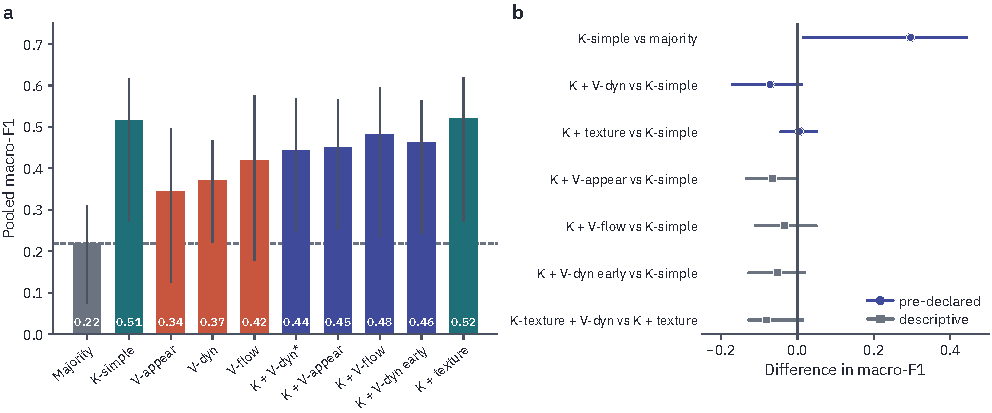
\includegraphics{fig3_results.pdf}
\caption{(a) Pooled macro-F1 of the majority class, the kinematic models (teal), the video-only models (red) and the fusion models (blue). Error bars are 95\% user-level bootstrap intervals; the dashed line is the majority-class score; * marks the pre-declared primary multimodal model. (b) Paired differences in macro-F1 with 95\% user-level bootstrap intervals. Circles are the three comparisons declared before the experiment; squares are descriptive comparisons.}
\label{fig:results}
\end{figure}

For comparison with the literature, \citet{zia2018rmis} report 88.2\% accuracy for Suturing under LOUO with approximate-entropy features. That figure is not directly comparable with ours. With 39 pooled predictions, accuracy moves in steps of 2.56 percentage points and 88.2\% is not attainable, so the published evaluation must have used a different trial set or a different aggregation, and it reports accuracy rather than macro-F1. The near-perfect results reported for deep networks on JIGSAWS mostly use LOSO, in which the test surgeon contributes training trials \citep{fawaz2018cnn, funke2019video}. Our bootstrap intervals, which are between about 0.25 and 0.4 wide in macro-F1, illustrate how little eight surgeons can resolve \citep{varoquaux2018cv}: a single surgeon changing class can move macro-F1 by more than 0.1.

\subsection{Analysis of successes and failures}

Figure~\ref{fig:confusion} shows where the errors occur. All three kinematic and multimodal models recognise novices well (F1 \FNMOne{} for K-simple) and intermediates moderately (F1 \FIMOne{}), but they almost never recognise experts (F1 \FEMOne{}). Of the ten expert trials, K-simple labels five as novice, four as intermediate and one as expert. Figure~\ref{fig:users} breaks this down by surgeon. The novices B and G and the intermediates C and F are largely classified correctly (4/5 or 5/5), whereas expert D has one correct trial in every kinematic model and expert E has none in any of them. The failure has a structural cause. When one expert is held out, the training set contains exactly one expert surgeon, so the classifier can learn what that surgeon looks like rather than what experts have in common, and the identity probe shows that this is easy: K-simple identifies the surgeon from a single trial with balanced accuracy \IdKSimple{} against a chance level of 0.125 (Figure~\ref{fig:audit}a). The pace of the trial does not help either. The median expert trial lasts \DurE{}\,s, close to the intermediate median of \DurI{}\,s and well below the novice median of \DurN{}\,s (Figure~\ref{fig:data}a), so duration separates novices from trained surgeons but cannot separate the two trained classes.

\begin{figure}[htbp]
\centering
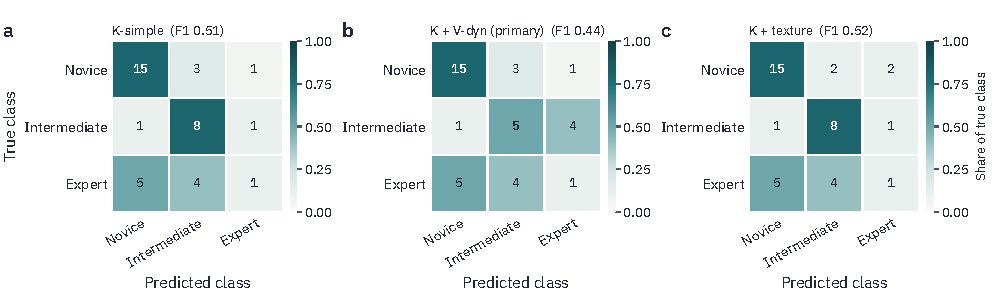
\includegraphics{fig4_confusion.pdf}
\caption{Pooled confusion matrices of (a) K-simple, (b) the primary multimodal model and (c) K-simple with motion texture. Numbers are trial counts; colour is the share of the true class.}
\label{fig:confusion}
\end{figure}

\begin{figure}[htbp]
\centering
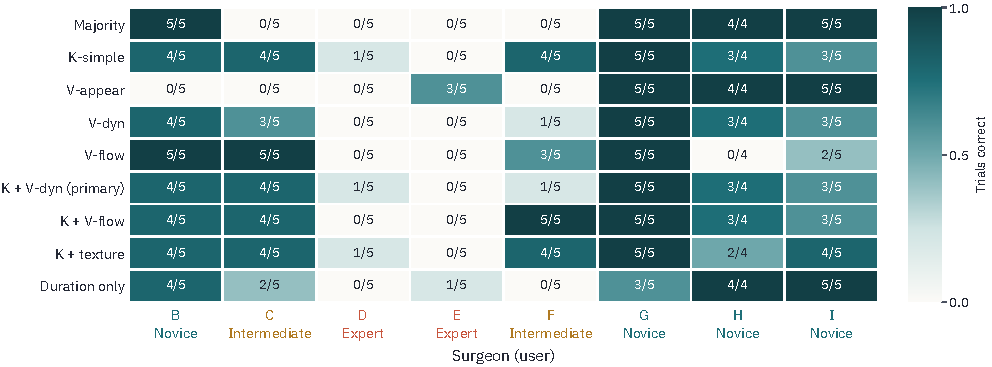
\includegraphics{fig5_users.pdf}
\caption{Correct trials per held-out surgeon for selected models. Each column is one LOUO fold; the label below gives the surgeon's skill level. Expert D and expert E are the dominant failure for every model except V-appear, which instead fails on novice B and both intermediates.}
\label{fig:users}
\end{figure}

Figure~\ref{fig:cases} shows the same pattern for single trials. The clearest successes are trials whose pace is typical of their class. Novice trial G001 lasts \CaseGZeroOneDur{}\,s and is labelled novice with probability \CaseGZeroOnePPred{}, and intermediate trial C004 lasts \CaseCZeroFourDur{}\,s and is labelled intermediate with probability \CaseCZeroFourPPred{}. The two experts fail in opposite directions, which is what a model that has learned one person rather than a class would do. When E is held out, the only training expert is D, whose trials last \DurRangeD{}\,s. E's trials last \DurRangeE{}\,s, so they probably look slow for an expert, and all five are labelled novice; E001 (\CaseEZeroOneDur{}\,s) receives a novice probability of \CaseEZeroOnePPred{} and an expert probability of only \CaseEZeroOnePTrue{}. When D is held out, the only training expert is E, so the fastest training trials belong to the intermediates (\DurRangeCF{}\,s), and four of D's five trials are labelled intermediate. This includes D005, the shortest trial in the dataset at \CaseDZeroFiveDur{}\,s, which receives an intermediate probability of \CaseDZeroFivePPred{} and an expert probability of \CaseDZeroFivePTrue{}. Not every error follows from duration. The last two trials of novice I are labelled intermediate with high confidence although both last about two minutes (I005, \CaseIZeroFiveDur{}\,s, intermediate probability \CaseIZeroFivePPred{}), so the model also responds to K-simple features other than the trial length.

\begin{figure}[htbp]
\centering
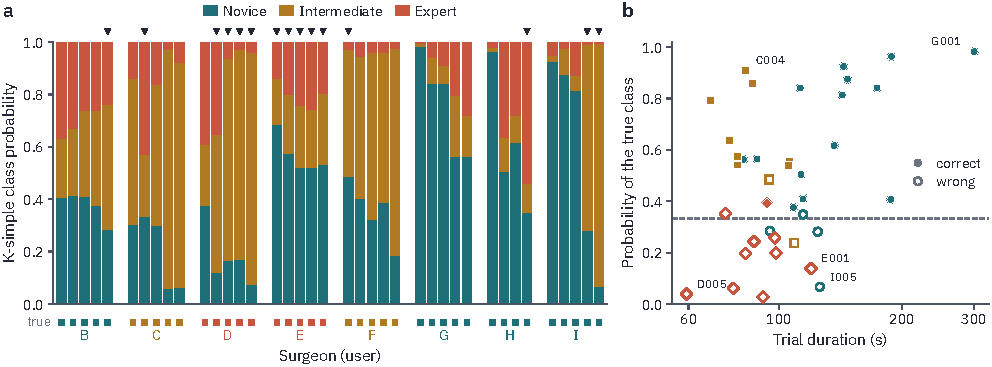
\includegraphics{fig7_cases.pdf}
\caption{Trial-level predictions of K-simple. (a) Class probabilities for every trial, grouped by held-out surgeon; squares below the bars give the true class and triangles mark wrong predictions. (b) Probability assigned to the true class against trial duration (log scale); filled markers are correct predictions, open markers are errors, and the dashed line is chance (1/3). The labelled trials are discussed in the text.}
\label{fig:cases}
\end{figure}


The pace audit shows how much of the kinematic signal is speed. A classifier on duration alone (C1) reaches macro-F1 \FCOne{}, well above the majority class, and the median absolute correlation of the K-simple features with log duration is \PaceKSimple{}. When every K-simple feature is residualised on log duration inside the training folds (C2), macro-F1 falls from \FMOne{} to \FCTwo{}, and the same happens with the texture block added (C2t, \FCTwoT{}). The skill information that K-simple transfers to new surgeons is therefore largely carried by how long the trial takes and by the quantities that scale with it (Figure~\ref{fig:audit}b). This is plausible for the novice versus trained distinction in a bench-top task, where trained surgeons are faster, but it is not a measure of quality and it explains why the expert class is missed.

\begin{figure}[htbp]
\centering
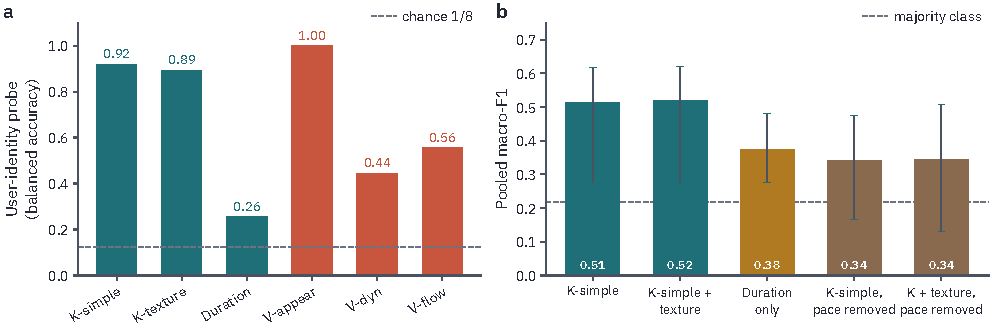
\includegraphics{fig6_audit.pdf}
\caption{Shortcut audit. (a) Balanced accuracy of an eight-way surgeon-identity probe on each feature block (stratified five-fold over trials); the dashed line is chance. (b) Macro-F1 of the kinematic models compared with a duration-only classifier and with the same kinematic features after removing their linear dependence on log duration inside each training fold.}
\label{fig:audit}
\end{figure}

The video results are explained by the same two mechanisms. V-appear identifies the surgeon perfectly (balanced accuracy \IdVAppear{}), yet as a skill classifier it reaches only \FMTwoA{}, and Figure~\ref{fig:users} shows the pattern expected of a block that recognises recording sessions: it is correct for all trials of the novices G, H and I and for three trials of expert E, but wrong for every trial of novice B and of both intermediates. The occasional success on expert E is therefore unlikely to reflect skill. V-dyn, designed to cancel static appearance, carries much less identity (\IdVDyn{}) but is strongly tied to pace: its median absolute correlation with log duration is \PaceVDyn{}, higher than that of K-simple. It thus adds a noisier copy of information the kinematic model already has. Late fusion with equal weights then hurts whenever the video classifier errs on a surgeon that kinematics gets right. The clearest case is intermediate F, for whom K-simple is correct on 4 of 5 trials and V-dyn on 1 of 5; after averaging, the fused model is correct on only \UFMThree{} (Figure~\ref{fig:users}). V-flow complements kinematics on F (fused \UFMThreeC{}) but fails completely on novice H, so its fusion again ends below kinematics alone.

The motion-texture improvement failed for a reason that can be seen in the features. The log dimensionless jerk of each instrument correlates with log duration at $|r| = \PaceKTextureMax{}$, which agrees with the known sensitivity of dimensionless jerk to movement duration \citep{hogan2009smoothness}, and the texture block identifies the surgeon almost as well as K-simple does (\IdKTexture{}). The ten texture features therefore largely duplicate the pace and identity information that K-simple already contains. Our block is also much smaller than the bank used by \citet{zia2018rmis}, who computed approximate entropy on every kinematic channel; we did not test the larger bank, because it was not part of the pre-declared protocol and choosing it after seeing these results would bias the comparison.

\subsection{Implementation and configuration details}

The inner LOUO selection chose strong regularisation in most folds ($C$ between 0.01 and 0.1 in seven of eight folds for K-simple), which is consistent with the small number of training surgeons. For V-appear the inner loop chose four principal components in six of eight folds. One inner fold was skipped in each of the outer folds C, D, E and F, as described in the protocol. Per-fold accuracy, averaged over surgeons, is \FoldAccMOne{} $\pm$ \FoldSdMOne{} (mean $\pm$ SD) for K-simple, and this per-fold spread is the reason we report pooled metrics with user-level intervals rather than a mean over folds. The code is organised as one module per stage (\texttt{data.py}, \texttt{features\_kin.py}, \texttt{features\_video.py}, \texttt{evaluate.py}), and \texttt{run\_all.py} reproduces every model, prediction file and statistic from the raw data in about five minutes; \texttt{make\_tables.py} and \texttt{make\_figures.py} regenerate the tables and figures of this report from the saved results without retraining.

\section{Conclusion and discussion}

\subsection{Summary of findings}

We classified the skill level of JIGSAWS Suturing trials as novice, intermediate or expert under the official leave-one-user-out protocol, following the experiment prescribed for this topic and a protocol that fixed every model and comparison before the first result. Simple trial-level kinematic statistics clearly beat the majority class (macro-F1 \FMOne{} against \FMZero{}, exact permutation $p = \PMOne{}$). Video features from sampled frames did not perform above chance on their own, and fusing them with kinematics, by late or early fusion, did not improve on kinematics alone; the pre-declared primary fusion scored \FMThree{}. The focused improvement, motion-texture features in the spirit of the background reference, left macro-F1 essentially unchanged at \FMFour{}. The shortcut audit explains most of this pattern. The transferable signal in the kinematic statistics is largely the pace of the trial, which separates novices from trained surgeons but not intermediates from experts, and with only two experts the model cannot learn what the two have in common, so the expert class is almost never recognised. The whole-frame appearance features identify the surgeon perfectly while carrying no transferable skill signal, and the scene-dynamics features mostly repeat the pace information.

The principal design choices follow from the size of the problem. With eight surgeons, and two in each trained class, we used linear models with strong, nested regularisation and frozen pretrained features rather than trained deep networks, and we reported pooled macro-F1 with user-level bootstrap intervals and an exact user-level permutation test, because per-fold macro-F1 is undefined when each fold contains one class. These choices make the results honest about their uncertainty, at the price of wide intervals that cannot resolve differences smaller than about 0.1 to 0.2 in macro-F1.

\subsection{Strengths and weaknesses}

The main strength of the study is that its conclusions do not depend on choices made after seeing the results. The folds are the official ones, the held-out surgeon never touches any fitted quantity, every model was evaluated once, and negative results are reported alongside positive ones. The audit also shows which information the classifier actually uses, which matters for any clinical use of such a system. Section~\ref{sec:differences} lists four ways in which the approach differs from the background reference and related work; for the conclusions of this study, the most important were the surgeon-level treatment of uncertainty and the direct measurement of the identity and pace shortcuts.

The method also has clear weaknesses. The method works best for what pace can reveal, namely telling a novice from a trained surgeon on a standardised bench-top task, and it is likely to fail whenever trained surgeons differ in quality rather than speed, as the expert class shows. The models are trained on seven surgeons, so a single atypical surgeon can dominate a fold, and the self-reported skill label measures hours of practice rather than observed performance. The video features describe whole frames and do not look at the needle, the thread or the tissue, which is where an observer would see differences in quality that kinematics cannot capture. Finally, equal-weight late fusion is a crude combination rule that lets a weak modality pull down a stronger one.

\subsection{Future directions}

The most effective step would be more surgeons, for example by training on all three JIGSAWS tasks with the held-out surgeon removed from each, or by adding other datasets, because the expert class cannot be learned from one training surgeon. Separating intermediates from experts probably requires features that are less tied to pace, such as gesture-level timing and error events or movement quality normalised by duration, and the identity probe and pace controls introduced here can serve as a check on any such feature. On the video side, features computed in a region around the instrument tips or on the final state of the suture could capture tissue handling and product quality, which neither the kinematics nor our whole-frame descriptors observe. A fusion weight chosen inside the training folds, or a fusion rule that defers to the stronger modality, would also avoid the dilution observed here. Any of these extensions should keep the strict LOUO protocol and the written pre-registration, since the small number of surgeons makes post-hoc choices easy to overfit.

\subsection*{AI tool declaration}

We used Claude Code with two Anthropic models, Claude Fable 5.1 and Claude Opus 5.5, to plan the experiments, write and debug the code, run the experiments, produce the figures and tables, and draft and edit this report and the slides. The group reviewed the code, the results and the text, and is responsible for the content and quality of the submitted work.


\small
\bibliographystyle{unsrtnat}
\bibliography{../report/references}

\end{document}
